\documentclass[12pt,a4paper]{article}
\usepackage{fontspec}
\setmainfont{Times New Roman}
\setsansfont{Arial}
\setmonofont{Courier New}
\usepackage[provide=*,english,romanian]{babel}
\usepackage{amsmath,amssymb,graphicx,geometry,setspace}
\usepackage{fancyhdr,caption,float,listings,xcolor,booktabs,longtable,array,calc}
\usepackage{subcaption,etoolbox,upquote}
\usepackage[unicode,hidelinks]{hyperref}
\geometry{top=2cm,bottom=2cm,left=2.5cm,right=2.5cm}
\setstretch{1.5}
\setlength{\parindent}{0pt}
\setlength{\parskip}{5pt}
\makeatletter
\renewcommand\section{\@startsection{section}{1}{0pt}{16pt}{7pt}{\normalfont\Large\bfseries}}
\renewcommand\subsection{\@startsection{subsection}{2}{0pt}{12pt}{5pt}{\normalfont\large\bfseries}}
\renewcommand\subsubsection{\@startsection{subsubsection}{3}{0pt}{9pt}{4pt}{\normalfont\normalsize\bfseries}}
\makeatother
\setcounter{secnumdepth}{-1}
\pagestyle{fancy}
\fancyhf{}
\rfoot{\thepage}
\renewcommand{\headrulewidth}{0pt}
\setlength{\headheight}{15pt}
\captionsetup{font=small,labelfont=bf,skip=6pt,justification=raggedright,singlelinecheck=false}
\captionsetup[figure]{position=above}
\lstset{language=C,basicstyle=\ttfamily\fontsize{9.5}{11.5}\selectfont,
  columns=fullflexible,showstringspaces=false,tabsize=2,numbersep=8pt,
  frame=single,rulecolor=\color{black!35},breaklines=true,keepspaces=true,
  xleftmargin=4pt,xrightmargin=4pt,aboveskip=8pt,belowskip=8pt}
\AtBeginEnvironment{lstlisting}{\singlespacing}
\AtBeginEnvironment{longtable}{\small\singlespacing}
\setlength{\emergencystretch}{3em}
\providecommand{\tightlist}{\setlength{\itemsep}{0pt}\setlength{\parskip}{0pt}}
\providecommand{\passthrough}[1]{#1}
\providecommand{\pandocbounded}[1]{#1}
\hypersetup{pdftitle={Sisteme de operare — Laborator 13},pdfauthor={Tacu Igor}}
\clubpenalty=10000
\widowpenalty=10000
\displaywidowpenalty=10000
\begin{document}
\begin{titlepage}
\thispagestyle{empty}
\begin{center}
\setstretch{1.18}

\includegraphics[width=0.23\textwidth]{scripts/report-style/utm-logo.png}\\[12pt]
\textbf{MINISTERUL EDUCAȚIEI ȘI CERCETĂRII}\\
\textbf{AL REPUBLICII MOLDOVA}\\[4pt]
\textbf{Universitatea Tehnică a Moldovei}\\
\textbf{Facultatea de Calculatoare, Informatică și Microelectronică}\\
\textbf{Departamentul Inginerie Software și Automatică}\\[36pt]
{\fontsize{22}{26}\selectfont\textbf{Raport}}\\[10pt]
Lucrare de laborator nr. 13\\[8pt]
\textbf{\large Sisteme de operare}\\[24pt]
\textbf{Tema:} Implementarea semafoarelor în kernel-ul xv6
\end{center}
\vfill
\begin{flushright}
\setstretch{1.25}
Realizat de:\\
stud. gr. FAF-242, Tacu Igor\\[24pt]
Verificat de:\\
Reițman Patricia
\end{flushright}
\vfill
\begin{center}\textbf{Chișinău – 2026 }\end{center}
\end{titlepage}

\setcounter{page}{1}
\section{Scopul lucrării}\label{scopul-lucrux103rii}

Implementarea operațiilor sem\_init, sem\_down și sem\_up în xv6 și
verificarea lor pentru ordonarea proceselor și protejarea liniilor
afișate.

\section{Sarcina lucrării}\label{sarcina-lucrux103rii}

\begin{itemize}
\tightlist
\item
  Înregistrarea apelurilor 24--26, a declarațiilor și a stub-urilor user
  și reproducerea Check 1.
\item
  Implementarea contorului, a spinlock-ului și a protocolului
  sleep\_prepare--sleep--wakeup.
\item
  Verificarea semtest și compararea mix fără blocare și cu blocare;
  păstrarea rezultatelor și a capturilor disponibile.
\end{itemize}

\section{Considerații teoretice}\label{consideraux21bii-teoretice}

Semaforul din kernel combină un contor protejat de spinlock cu o coadă
logică de așteptare identificată printr-un canal. Un proces fără permis
trebuie să înregistreze canalul și să elibereze spinlock-ul înainte de
somn. Trezirea este o invitație de a reîncerca; contorul se verifică
într-o buclă deoarece alți competitori pot consuma permisul.

\section{Implementare. Rezultate
practice}\label{implementare.-rezultate-practice}

\subsection{Implementation and
environment}\label{implementation-and-environment}

The canonical modified xv6 tree is
\href{https://github.com/igortacu/OS/blob/main/xv6}{../xv6}. The three
system calls are {\ttfamily\fontsize{10}{12}\selectfont sem\_init} (24),
{\ttfamily\fontsize{10}{12}\selectfont sem\_down} (25) and
{\ttfamily\fontsize{10}{12}\selectfont sem\_up} (26); the existing
{\ttfamily\fontsize{10}{12}\selectfont sync} (22) and
{\ttfamily\fontsize{10}{12}\selectfont trace} (23) remain available.
Eight semaphore slots, IDs 0--7, are shared by all processes.

The source was compiled and tested on the Ubuntu server using the RISC-V
cross compiler and QEMU with
{\ttfamily\fontsize{10}{12}\selectfont CPUS=3}. The
\href{https://github.com/igortacu/OS/blob/main/Lab13/evidence/build-final.txt}{final
build log},
\href{https://github.com/igortacu/OS/blob/main/Lab13/evidence/build-check1.txt}{intermediate
build log},
\href{https://github.com/igortacu/OS/blob/main/Lab13/evidence/execution.txt}{QEMU
execution log} and
\href{https://github.com/igortacu/OS/blob/main/Lab13/evidence/results.json}{checked
results} retain the actual evidence. Tests were performed on 18 November
2026. Both builds complete; their logs retain the linker warnings about
RWX LOAD segments in
{\ttfamily\fontsize{10}{12}\selectfont kernel/kerne\allowbreak{}l} and
{\ttfamily\fontsize{10}{12}\selectfont user/\_forkte\allowbreak{}st}.
Intermediate output and final successful output are identified
separately.

The implementation follows the Lab 13 handout and this tree's
{\ttfamily\fontsize{10}{12}\selectfont sleep\_prepar\allowbreak{}e(chan)}
followed by {\ttfamily\fontsize{10}{12}\selectfont sleep()} API. It does
not use the older
{\ttfamily\fontsize{10}{12}\selectfont sleep(chan, lock)} interface. The
only canonical kernel tree is committed under
{\ttfamily\fontsize{10}{12}\selectfont xv6/}; the incomplete Check 1
tree is generated outside the repository by
\href{https://github.com/igortacu/OS/blob/main/Lab13/prepare-check1.py}{prepare-check1.py}.

\subsection{Part 1 --- Syscall numbers, declarations and
stubs}\label{part-1-syscall-numbers-declarations-and-stubs}

Registration touches these files:

{\def\LTcaptype{table} % do not increment counter
\begin{longtable}[]{@{}
  >{\raggedright\arraybackslash}p{(\linewidth - 2\tabcolsep) * \real{0.5000}}
  >{\raggedright\arraybackslash}p{(\linewidth - 2\tabcolsep) * \real{0.5000}}@{}}
\toprule\noalign{}
\begin{minipage}[b]{\linewidth}\raggedright
File
\end{minipage} & \begin{minipage}[b]{\linewidth}\raggedright
Role
\end{minipage} \\
\midrule\noalign{}
\endhead
\bottomrule\noalign{}
\endlastfoot
\href{https://github.com/igortacu/OS/blob/main/xv6/kernel/syscall.h}{syscall.h}
& Reserve numbers 24--26 \\
\href{https://github.com/igortacu/OS/blob/main/xv6/user/user.h}{user.h}
& Declare the three user functions \\
\href{https://github.com/igortacu/OS/blob/main/xv6/user/usys.pl}{usys.pl}
& Generate the RISC-V ecall stubs \\
\href{https://github.com/igortacu/OS/blob/main/xv6/kernel/syscall.c}{syscall.c}
& Declare handlers, register dispatcher entries and trace names \\
\href{https://github.com/igortacu/OS/blob/main/xv6/Makefile}{Makefile} &
Link sem.o and put semtest, mix and supplemental semcheck on the disk \\
\end{longtable}
}

\par\noindent\begin{minipage}{\linewidth}

\begin{lstlisting}[language=C]
#define SYS_sem_init 24
#define SYS_sem_down 25
#define SYS_sem_up 26

int sem_init(int, int);
int sem_down(int);
int sem_up(int);
\end{lstlisting}

\end{minipage}\par

\subsubsection{Check 1 --- deliberately incomplete
dispatcher}\label{check-1-deliberately-incomplete-dispatcher}

The disposable
{\ttfamily\fontsize{10}{12}\selectfont /root/os-lab\allowbreak{}13-check1}
build includes the user stubs but omits all three semaphore handlers
from the dispatcher table. The recorded first lines were:

\par\noindent\begin{minipage}{\linewidth}

\begin{lstlisting}
semtest
3 semtest: unknown sys call 24
4 semtest: unknown sys call 25
child: I ran after the parent
parent: done, I let the child go
\end{lstlisting}

\end{minipage}\par

The child did not block because
{\ttfamily\fontsize{10}{12}\selectfont sem\_down} was unrecognized.
Subsequent ping/pong text is interleaved with unknown syscall errors.
The handout's {\ttfamily\fontsize{10}{12}\selectfont semtest} prints
{\ttfamily\fontsize{10}{12}\selectfont semtest: OK} even at this stage,
since it does not check the return values; therefore that final string
alone is insufficient evidence of correct semaphores. The validation
runner checks the errors and the child-before-parent ordering in Check
1, then checks the entire expected ordered output in Check 2.

\subsubsection{Native Terminal evidence --- Check
1}\label{native-terminal-evidence-check-1}

\par\medskip\noindent\begin{minipage}{\linewidth}\setstretch{1.0}
\captionof*{figure}{Figura 1. Native Terminal capture: boot of the intermediate Check 1 tree, unregistered semaphore calls and the child running before the parent.}
\centering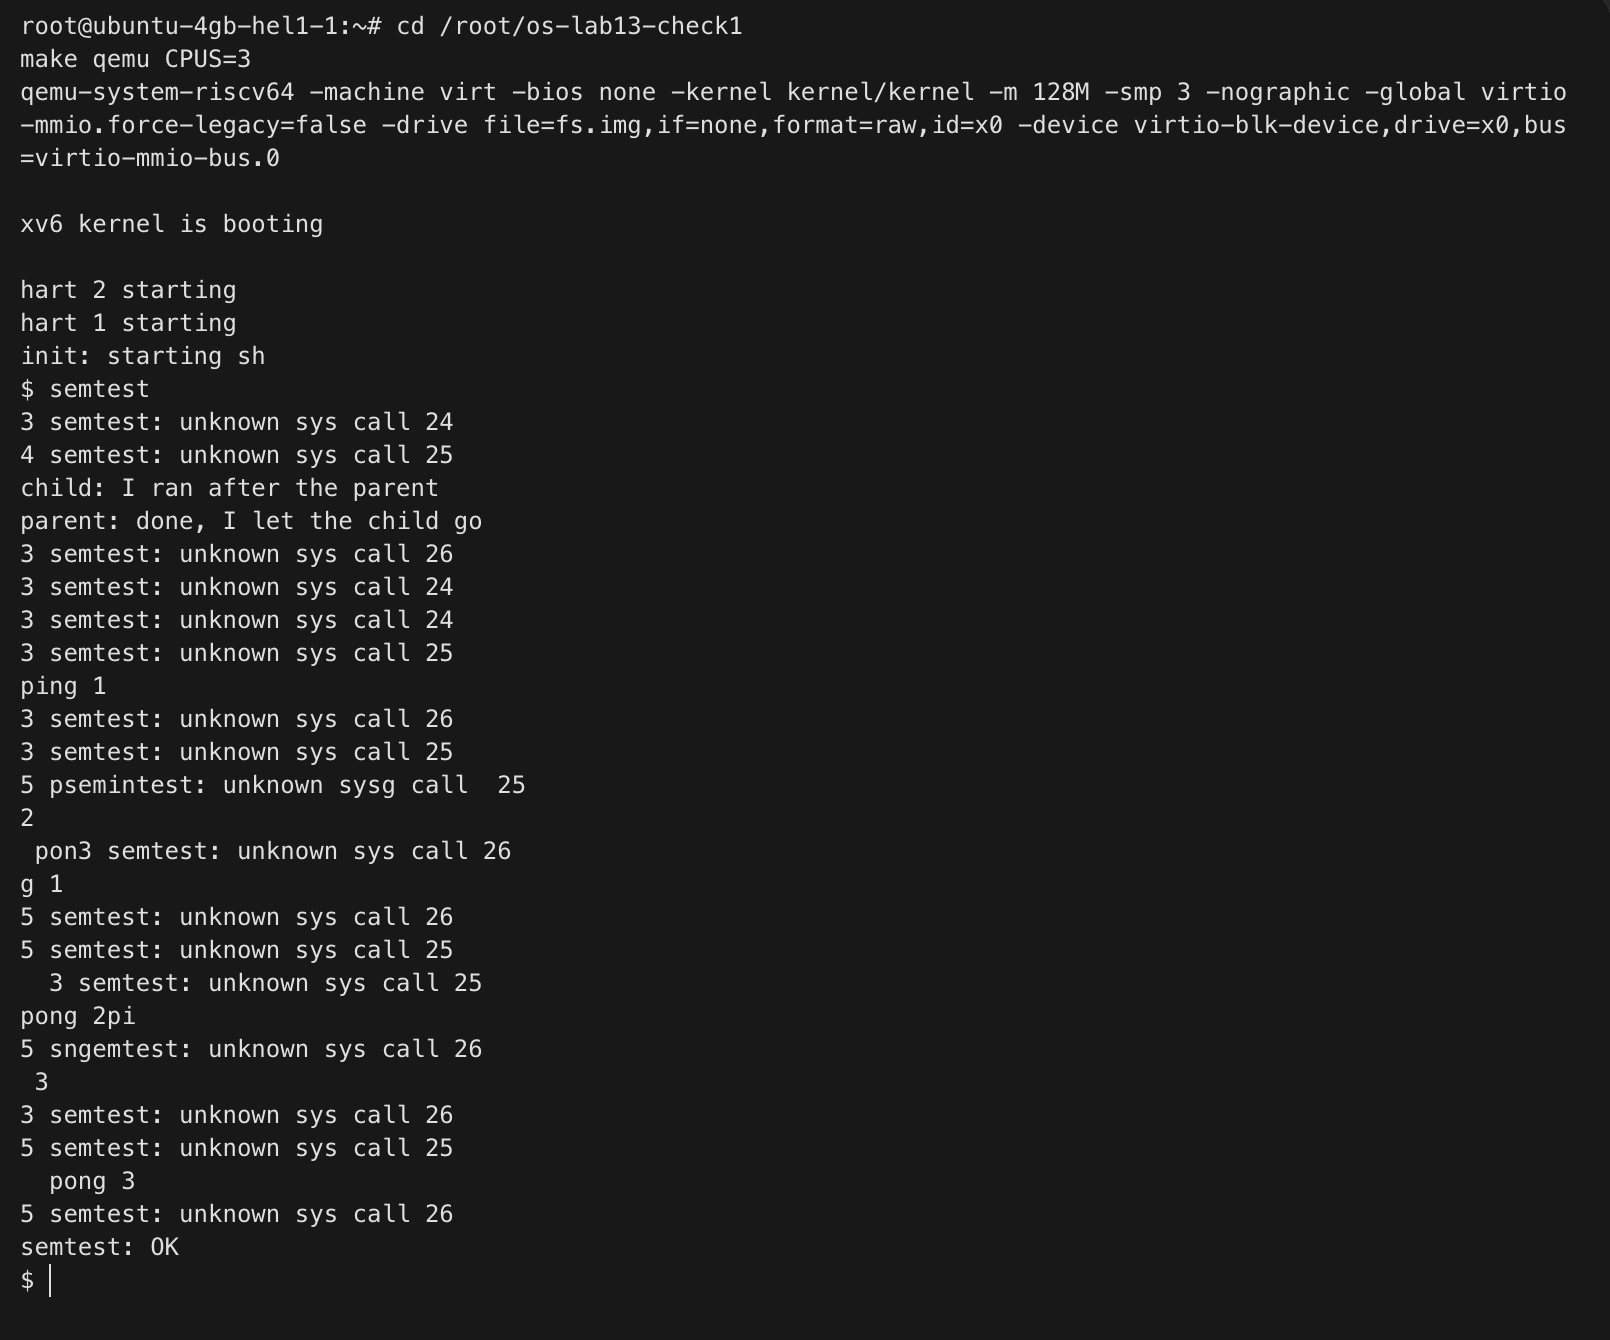
\includegraphics[width=\linewidth,height=0.67\textheight,keepaspectratio]{Lab13/evidence/screenshots/lab13-check1-terminal.png}
\end{minipage}\par\medskip

The supplied capture shows
{\ttfamily\fontsize{10}{12}\selectfont /root/os-lab\allowbreak{}13-check1}
booting with three CPUs. Calls 24 and 25 are initially rejected, and the
child's line appears before the parent's line. Later unknown-call
diagnostics and ping/pong text interleave because the operations do not
synchronize either process. The trailing
{\ttfamily\fontsize{10}{12}\selectfont semtest: OK} is printed by the
utility despite these failures and is not evidence of the final kernel
implementation. This capture documents the deliberately incomplete stage
only; the final implementation's separate automated validation is
retained in the execution log.

\subsection{Part 2 --- Kernel semaphore
operations}\label{part-2-kernel-semaphore-operations}

Source:
\href{https://github.com/igortacu/OS/blob/main/xv6/kernel/sem.c}{kernel/sem.c}.
Each slot has a protected integer count and a spinlock. The static array
begins zeroed, as permitted by the handout's spinlock representation.

{\ttfamily\fontsize{10}{12}\selectfont sem\_init} rejects IDs outside
0--7 and negative initial values. It replaces the count while holding
the slot lock. In these demonstrations, initialization occurs before
users begin waiting. The shared table is a teaching interface: it has no
ownership, access control, allocation/destruction protocol or FIFO
fairness guarantee. Reinitializing an actively used semaphore is outside
the experiments and is not a safe reset protocol for existing waiters.

The blocking operation is:

\par\noindent\begin{minipage}{\linewidth}

\begin{lstlisting}[language=C]
acquire(&s->lock);
while (s->value == 0) {
  sleep_prepare(s);
  release(&s->lock);
  sleep();
  acquire(&s->lock);
  if (killed(myproc())) {
    release(&s->lock);
    return -1;
  }
}
s->value--;
release(&s->lock);
\end{lstlisting}

\end{minipage}\par

Registering the channel while holding the semaphore lock closes the
window for a lost semaphore post. If
{\ttfamily\fontsize{10}{12}\selectfont sem\_up} runs after registration
but before {\ttfamily\fontsize{10}{12}\selectfont sleep},
{\ttfamily\fontsize{10}{12}\selectfont wakeup} clears the registered
channel and this xv6 implementation's
{\ttfamily\fontsize{10}{12}\selectfont sleep()} returns without putting
the process to sleep. Otherwise the process becomes sleeping and is
scheduled away. Once awakened, it reacquires the lock and retries the
predicate; it does not busy-poll the count while blocked.

The posting operation, under the same slot lock, is:

\par\noindent\begin{minipage}{\linewidth}

\begin{lstlisting}[language=C]
if (s->value == 0x7fffffff) {
  release(&s->lock);
  return -1;
}
s->value++;
wakeup(s);
release(&s->lock);
\end{lstlisting}

\end{minipage}\par

The upper-bound check additionally prevents signed integer overflow. The
handlers are registered with names in the existing Lab 10 tracer, so
tracing a new semaphore call produces its name rather than an absent
name entry.

\subsubsection{Check 2 --- order and
ping/pong}\label{check-2-order-and-pingpong}

The final implementation passed ten successive executions with this
complete sequence:

\par\noindent\begin{minipage}{\linewidth}

\begin{lstlisting}
parent: done, I let the child go
child: I ran after the parent
ping 1
  pong 1
ping 2
  pong 2
ping 3
  pong 3
semtest: OK
\end{lstlisting}

\end{minipage}\par

Semaphore 0 starts at zero. The child waits while the parent pauses for
ten ticks; the parent prints before posting the permit. Semaphores 1 and
2 start at one and zero, respectively, and exchange the turn between
ping and pong. The runner checks every line and its order in all ten
repetitions, not just the final success label.

\subsection{Part 3 --- Semaphore as a line
lock}\label{part-3-semaphore-as-a-line-lock}

Source:
\href{https://github.com/igortacu/OS/blob/main/xv6/user/mix.c}{user/mix.c}.

\par\noindent\begin{minipage}{\linewidth}

\begin{lstlisting}[language=C]
for (int k = 0; k < 5; k++) {
  if (uselock)
    sem_down(3);
  for (char *p = s; *p; p++)
    write(1, p, 1);
  if (uselock)
    sem_up(3);
}
\end{lstlisting}

\end{minipage}\par

Two unlocked runs were recorded with three QEMU CPUs. Both showed mixed
A/b lines; the raw output is preserved without reconstruction in the
execution log. The checker verifies a total of 150
{\ttfamily\fontsize{10}{12}\selectfont A} characters and 150
{\ttfamily\fontsize{10}{12}\selectfont b} characters for each run, so
interleaving is distinguished from lost output. Each process emits five
newlines as well.

Two locked runs each contained exactly five lines of 30
{\ttfamily\fontsize{10}{12}\selectfont A} characters and five lines of
30 {\ttfamily\fontsize{10}{12}\selectfont b} characters. In the final
saved validation, both locked runs grouped all A lines before all b
lines. Scheduling can also switch processes between complete lines. The
requirement is: the semaphore protects each complete line, not the
entire five-line batch or a prescribed process order.

The required four Observe answers are also provided in
\href{https://github.com/igortacu/OS/blob/main/Lab13/notes.txt}{notes.txt}:

\begin{enumerate}
\def\labelenumi{\arabic{enumi}.}
\tightlist
\item
  One line costs 31 writes: 30 letters and a newline. Each write is a
  separate opportunity for the processes to interleave.
\item
  {\ttfamily\fontsize{10}{12}\selectfont sem\_down(3)} before the byte
  loop and {\ttfamily\fontsize{10}{12}\selectfont sem\_up(3)} after it
  make the whole line a critical section.
\item
  {\ttfamily\fontsize{10}{12}\selectfont wakeup(s)} can awaken several
  waiters for one available permit. A competing waiter may consume it
  first, so the condition must be checked with
  {\ttfamily\fontsize{10}{12}\selectfont while}.
\item
  The semaphore spinlock must be released before sleeping so a posting
  process can acquire it and make progress; sleeping with it held also
  violates the scheduler's spinlock constraints.
\end{enumerate}

\subsection{Additional checks and
reproduction}\label{additional-checks-and-reproduction}

The supplemental
\href{https://github.com/igortacu/OS/blob/main/xv6/user/semcheck.c}{user/semcheck.c}
verifies invalid IDs for all three calls, a negative initial count, the
overflow guard, consumption of two permits, release and successful
reaping of four waiting children, and killing/reaping a child blocked on
a zero-valued semaphore. It reported:

\par\noindent\begin{minipage}{\linewidth}

\begin{lstlisting}
semcheck: bounds and counting OK
semcheck: four waiting children released OK
semcheck: killed blocked child reaped OK
semcheck: OK
\end{lstlisting}

\end{minipage}\par

The finite killed-waiter test exercises an already blocked child; it is
not an exhaustive check of every possible kill/sleep interleaving. The
handout's wait protocol is retained. The original
{\ttfamily\fontsize{10}{12}\selectfont trace 32 grep hello README} check
and {\ttfamily\fontsize{10}{12}\selectfont usertests forkforkfork} also
passed after the kernel changes. Tracing syscall 26 with mask 67108864
printed {\ttfamily\fontsize{10}{12}\selectfont syscall sem\_up -> 0} and
allowed semtest to complete. Trace diagnostics can interleave with user
output and are retained as recorded.

Build the canonical implementation from
{\ttfamily\fontsize{10}{12}\selectfont xv6/} with
{\ttfamily\fontsize{10}{12}\selectfont make kernel/kerne\allowbreak{}l fs.img},
then {\ttfamily\fontsize{10}{12}\selectfont make qemu CPUS=3}. To
reproduce Check 1, run
{\ttfamily\fontsize{10}{12}\selectfont python3 Lab13/prepar\allowbreak{}e-check1.py /tmp/os-lab1\allowbreak{}3-check1}
from the repository root, build that disposable directory, and keep it
separate from the final tree. To repeat automated checks, use
{\ttfamily\fontsize{10}{12}\selectfont python3 Lab13/check-\allowbreak{}lab13.py /path/to/fin\allowbreak{}al/xv6 /path/to/che\allowbreak{}ck1 /path/to/new\allowbreak{}/evidence}.
The checker boots both trees and overwrites the evidence files in its
selected output directory.

\href{https://github.com/igortacu/OS/blob/main/Lab13/CAPTURES.md}{Native
capture commands} separate the intermediate failure from the final
passing implementation. Screenshots will be embedded with captions as
the live repetitions are captured; saved command logs are not presented
as native live screenshots.

\par\noindent\begin{minipage}{\linewidth}

\section{Concluzie}\label{concluzie}

Testele automate ale implementării finale au verificat ordinea
părinte--copil, alternarea ping/pong și liniile întregi cu semafor.
Captura Check 1 documentează etapa incompletă și nu trebuie confundată
cu probele native ale etapei finale, care urmează să fie adăugate.

\end{minipage}\par

\end{document}
